\documentclass{article}


\usepackage{PRIMEarxiv}
\usepackage{natbib}
\usepackage{multirow}
\usepackage{multirow}
\usepackage{multirow}
\usepackage[utf8]{inputenc} % allow utf-8 input
\usepackage[T1]{fontenc}    % use 8-bit T1 fonts
\usepackage{hyperref}       % hyperlinks
\usepackage{url}            % simple URL typesetting
\usepackage{booktabs}       % professional-quality tables
\usepackage{amsfonts}       % blackboard math symbols
\usepackage{nicefrac}       % compact symbols for 1/2, etc.
\usepackage{microtype}      % microtypography
\usepackage{lipsum}
\usepackage{fancyhdr}       % header
\usepackage{graphicx}       % graphics
\graphicspath{{media/}}     % organize your images and other figures under media/ folder
\usepackage{microtype}
\usepackage{graphicx}
\usepackage{subcaption}
\usepackage{booktabs}
\usepackage{amsmath}
\usepackage{amssymb}
\usepackage{mathtools}
\usepackage{amsthm}
\usepackage{float}
\pagestyle{fancy}
\thispagestyle{empty}
\rhead{ \textit{ }} 
\fancyhead[LO]{\small Mapper-GIN: Lightweight Structural Graph Abstraction for Corrupted 3D Point Cloud Classification}

\title{Mapper-GIN: Lightweight Structural Graph Abstraction for Corrupted 3D Point Cloud Classification}

\author{
  Jeongbin You \\
  Department of Mathematics \\
  Korea University \\
  \texttt{dbwjdqls03@gmail.com} \\
  \And
  Donggun Kim \\
  Department of Mathematics \\
  Korea University \\
  \texttt{dorage1105@korea.ac.kr} \\
  \And
  Sejun Park \\
  Department of Mathematics \\
  Korea University \\
  \texttt{safespot@korea.ac.kr} \\
  \And
  Seungsang Oh \\
  Department of Mathematics \\
  Korea University \\
  \texttt{seungsang@korea.ac.kr} \\
}

\begin{document}
\maketitle
\begin{abstract}
Robust 3D point cloud classification is often pursued by scaling up backbones or relying on specialized data augmentation. We instead ask whether structural abstraction alone can improve robustness, and study a simple topology-inspired decomposition based on the Mapper algorithm. We propose \emph{Mapper-GIN}, a lightweight pipeline that partitions a point cloud into overlapping regions using Mapper (PCA lens, cubical cover, and followed by density-based clustering), constructs a region graph from their overlaps, and performs graph classification with a Graph Isomorphism Network. On the corruption benchmark ModelNet40-C, Mapper-GIN achieves competitive and stable accuracy under Noise and Transformation corruptions with only 0.5M parameters. In contrast to prior approaches that require heavier architectures or additional mechanisms to gain robustness, Mapper-GIN attains strong corruption robustness through simple region-level graph abstraction and GIN message passing. Overall, our results suggest that region-graph structure offers an efficient and interpretable source of robustness for 3D visual recognition.
\end{abstract}


\section{Introduction}

The growing availability of 3D sensors has made point cloud recognition a core component in applications like autonomous systems~\cite{7583659, Kidono2011PedestrianRU}. Over the past years, a wide range of architectures have been proposed for point cloud classification. Pioneering pointwise models such as PointNet~\cite{pointnet2017} and PointNet++~\cite{qi2017pointnetplusplus} established strong baselines by processing points with permutation-invariant operators. To capture local geometric structures better, graph-based approaches such as DGCNN~\cite{dynamicgcnn2019} introduced dynamic graph construction in feature space, and RSCNN~\cite{liu2019rscnn} incorporated explicit geometric relations between points. More recently, transformer-style attention as in PCT~\cite{guo2021pct} has been used to capture longer-range dependencies, and projection-based pipelines such as SimpleView~\cite{goyal2021revisiting} have shown that surprisingly competitive representations can be obtained by projecting 3D points into 2D views.

Despite these advances, robustness remains a persistent issue. Models that perform well on clean benchmarks can degrade sharply under real-world artifacts such as occlusion and LiDAR density corruptions and background noise addition, which are commonly occurring corruptions. The ModelNet40-C~\cite{modelnetbench2022} benchmark makes this failure mode explicit by evaluating 3D classifiers under 15 corruption types with increasing severity. Current countermeasures, such as data augmentation or adversarial training, focus on data-driven generalization with expanded training distributions, rather than explicitly modeling the fundamental structural invariants of the shape.

To address this fragility, topological data analysis (TDA) provides a general mathematical tool for summarizing the ``shape'' of data in ways that are less sensitive to small perturbations. Originally applied in broad fields ranging from biology to materials science, TDA captures global structural invariants, such as connected components, loops, and voids, that persist across continuous deformations. With this potential, there has been a growing interest in integrating TDA with deep learning models. 
For example, \textit{PersLay}~\cite{carriere2018perslay} enables the vectorization of persistence diagrams, allowing topological features to be directly processed by neural networks. Similarly, \citet{hofer2017deep} introduced a method to learn topological signatures via deep learning, demonstrating improved performance in classification tasks.

One of the core techniques in TDA is the Mapper algorithm~\cite{mapper2007}, which summarizes a point cloud by grouping points into overlapping regions defined by a low-dimensional lens and cover, and then connecting regions that share points, producing a graph that reflects coarse global organization. Mapper is typically used for exploratory data analysis (EDA) and visualization, where the output graph is inspected by humans. For instance, it has been utilized as a visual aid to identify distinct breast cancer subgroups~\cite{nicolau2011topology} or to qualitatively analyze high-dimensional datasets in healthcare and sports~\cite{lum2013extracting}. We repurpose Mapper from an endpoint visualization into an intermediate representation for downstream machine learning tasks.

Concretely, we propose \emph{Mapper-GIN}, a lightweight pipeline that first lifts a point cloud to a structural graph representation via a Mapper region graph, and then applies a simple graph encoder for classification. By moving from dense point processing to a topology-inspired abstraction, we can exploit object-level connectivity with substantially fewer parameters than heavy geometric backbones. We instantiate the graph encoder with the Graph Isomorphism Network (GIN)~\cite{gin2019}, since its injective multiset aggregation is well suited for discriminating graph structures and thus aligns naturally with our goal of leveraging global connectivity patterns encoded in Mapper graphs.

Experiments on ModelNet40-C show that the proposed approach is particularly robust to transformation corruptions. We attribute this behavior to the fact that, although transformations such as rotations and non-linear warping can substantially change geometric appearance, they do not fundamentally alter the object’s underlying connectivity structure. Our Mapper construction, together with structure-aware aggregation, is designed to emphasize this structural signal, making the representation less sensitive to global coordinate changes than purely point-local descriptors. Moreover, the method remains competitively stable under noise corruptions, especially impulse noise, which we attribute to region-level pooling that mitigates the influence of isolated outliers. Taken together, these results suggest that stabilized structural representations can provide a parameter-efficient path to robustness in 3D point cloud classification.

\section{Background} \label{sec:Background}
\subsection{Mapper Graph}

Mapper~\cite{mapper2007} is a technique from TDA that summarizes the coarse structure of a dataset by constructing a graph (or, more generally, a simplicial complex) from a point cloud and a low‑dimensional lens function.
Rather than operating directly on all points in a high‑dimensional space, Mapper organizes data into overlapping regions and connects regions that share data points. 
The resulting graph captures how local regions are arranged and related, offering a structural overview of the dataset. See Figures~\ref{fig1} and~\ref{fig2}.

Formally, let $X\! =\! \{x_1,\dots,x_N\}$ be a finite metric space, typically a point cloud embedded in $\mathbb{R}^d$.
Mapper begins with a continuous function, called a \emph{filter} or \emph{lens},
$$ f : X \longrightarrow \mathbb{R}^m, $$
which assigns to each point a low-dimensional descriptor.
Typical choices include scalar functions such as density, eccentricity, or height, as well as multi-dimensional embeddings obtained from principal component analysis (PCA) or other dimensionality-reduction methods. 
The role of the lens is to emphasize the directions or attributes of the data along which we want to probe its structure.

\begin{figure}[t]
    \centering  
    
\includegraphics[width=0.5\linewidth]{fig1.pdf}
    \caption{\small Mapper graph construction algorithm}
    \label{fig1}
\end{figure}

Next, one chooses an open cover $\mathcal{U} = \{U_\alpha\}_{\alpha \in A}$ of the image $f(X) \subset \mathbb{R}^m$.
In practice, this cover is often realized as overlapping intervals when $m=1$, or overlapping boxes when $m>1$.
The cover parameters such as resolution (the number of cover elements) and gain (the overlap ratio) control the level of abstraction: finer covers yield more regions and a more detailed graph, while coarser covers emphasize global structure.

For each cover element $U_\alpha \in \mathcal{U}$, Mapper considers its pullback
$$ S_\alpha \;=\; f^{-1}(U_\alpha) \subset X, $$
namely, the subset of points whose lens values lie within $U_\alpha$.
Since each $S_\alpha$ may still contain multiple disconnected groups of points, Mapper further refines these pullbacks through clustering.
Applying a clustering algorithm (e.g., single linkage, $k$-means, or density-based methods like DBSCAN~\cite{ester1996density}) to $S_\alpha$ produces clusters $\{C_{\alpha,\beta}\}$, which represent locally coherent
regions of the data inside $U_\alpha$.

The final Mapper complex is obtained by treating each cluster $C_{\alpha,\beta}$ as a node in a graph and connecting nodes whose clusters overlap:
$$ (C_{\alpha,\beta},\, C_{\alpha',\beta'}) \text{ are adjacent} \ \Longleftrightarrow \ C_{\alpha,\beta} \cap C_{\alpha',\beta'} \neq \varnothing. $$
More generally, one may construct a higher-dimensional simplicial complex by taking the nerve of the family $\{C_{\alpha,\beta}\}$.
However, many applications including the present work focus on the $1$‑skeleton, referred to as the
\emph{Mapper graph}.
This graph captures how local clusters overlap across the cover and provides a coarse yet interpretable representation of the underlying data geometry and topology.

Historically, Mapper has been used primarily as an exploratory and visualization tool, revealing global patterns such as branches, loops, and flares in high‑dimensional datasets. 
A key conceptual aspect of Mapper is the separation between (1) point‑level representations, which may be as simple as the original coordinates, and (2) a higher‑level structural abstraction encoded by the graph defined through the choice of lens, cover, and clustering.

In this work, we exploit this separation by treating the Mapper graph as a region‑level scaffold for learning. Rather than directly relying on expressive point‑level encoders, we operate on Mapper‑induced regions and their connectivity, allowing lightweight encoders and graph neural networks to operate. 
The specific instantiation of the lens, cover, and clustering for 3D point clouds is detailed in Section~\ref{sec:mapper_abstraction}.

\subsection{Graph Isomorphism Network (GIN)}
Graph Neural Networks (GNN) generalize deep learning methods to graph-structured data by iteratively aggregating features from neighboring nodes to update node representations. 
Standard GNN variants, such as Graph Convolutional Networks (GCN)~\cite{gcn2017} and GraphSAGE~\cite{graphsage2017}, typically employ mean or max pooling as aggregation functions. 
However, such pooling operators are not injective; different multisets of the neighbor feature vectors of nodes can map to the same aggregated representation, making these models unable to distinguish certain topologically distinct graphs despite structural differences.
This limitation restricts the expressive power of such models, making them less powerful than the Weisfeiler–Lehman (WL) graph isomorphism test~\cite{weisfeiler1968reduction}, a classical iterative algorithm for distinguishing non‑isomorphic graphs through injective aggregation updates.

The Graph Isomorphism Network~\cite{gin2019} is designed to overcome this limitation by achieving maximal expressiveness among the class of GNNs, theoretically achieving the same discriminative power as the WL test. 
By employing a sum aggregator, which uses a Multi-layer Perceptron (MLP) to implement a universal and injective function over multisets of neighbor features, GIN preserves complete neighborhood information that non‑injective aggregators fail to capture. 
The node update in the $k$-th layer is given by:
$$ h_v^{(k)} = \text{MLP}^{(k)} \Big( (1 + \epsilon^{(k)}) \cdot h_v^{(k-1)} +\!\! \sum_{u \in \mathcal{N}(v)}\!\! h_u^{(k-1)} \Big) $$
where $h_v^{(k)}$ is the feature vector of node $v$ in layer $k$, $\mathcal{N}(v)$ denotes its neighbors, and $\epsilon^{(k)}$ is a learnable parameter or a fixed scalar that enhances the injectivity of the mapping.

In our framework, the Mapper algorithm converts a 3D point cloud into a region-based graph where nodes represent local clusters and edges denote overlaps between them. 
Since these structural features (e.g., loops, branches) carry critical information about the object's global shape, we adopt GIN as our graph encoder to fully exploit the topology encoded by Mapper.
GIN’s strong discriminative capacity ensures that subtle topological differences, even under localized corruptions, are effectively captured in the learned representation.

\begin{figure*}[t]
  \centering
  
\includegraphics[width=\linewidth]{fig2.pdf} 
  \caption{\small Examples of a clean point cloud and three representative corruptions from the ModelNet40-C dataset, along with their corresponding Mapper graphs. While noise and transformation tend to preserve the overall graph structure, density reduction often disrupts connectivity, leading to noticeable changes in the Mapper graph.}
  \label{fig2}
\end{figure*}

\section{Methods} \label{sec:Methods}
Our aim is not to design a heavy recognition architecture, but to examine how topology-inspired Mapper abstraction, combined with a lightweight point encoder, can improve robustness against common point cloud corruptions such as cutout and impulse noise.
We introduce \emph{Mapper-GIN-Base} and \emph{Mapper-GIN}, simple graph-based models driven by two core components rather than specialized geometric modules: (1) stable region-level decomposition of the input cloud via the Mapper algorithm, and (2) expressive structure-aware aggregation over the resulting graph using GIN.

The framework proceeds in three stages (Figure~\ref{fig3}): 
\begin{itemize} \itemsep0pt
\item Topological Abstraction: A PCA lens, cubical cover, and density-based clustering yield a Mapper graph capturing overlapping subregions of the point cloud.
\item Node-wise Point Encoding: Each sub-cloud is normalized to a local coordinate frame and encoded via a shallow MLP to produce node features.
\item Graph Classification: Node features are propagated through GIN layers, regularized with DropEdge and feature dropout, followed by global pooling for classification.
\end{itemize} 
Despite its simplicity, this modular pipeline effectively leverages coarse structural cues to enhance robustness across diverse corruptions.

\subsection{Mapper Graph For Topological Abstraction} \label{sec:mapper_abstraction}
Let $X = \{x_1,\dots,x_N\} \subset \mathbb{R}^3$ denote the input point cloud.
Following the Mapper framework~\cite{mapper2007}, we construct a graph $G=(V,E)$ (Figure~\ref{fig2}) by sequentially applying (1) a lens map, (2) a cover over the lens space, and (3) clustering within each pullback set.
In our context, the goal is not to compute explicit topological invariants, but to obtain a stable region‑wise scaffold that supports robust feature aggregation under various corruptions.

\paragraph{Lens function.}
We adopt a lightweight PCA embedding $f_{\mathrm{PCA}} : X \to \mathbb{R}^3$ defined as
$$ f_{\mathrm{PCA}}(x) = W^\top(x-\mu), $$
where $\mu$ is the sample mean and $W$ contains the principal directions.
PCA serves as a coarse but computationally efficient lens that imposes a global coordinate structure for partitioning the point cloud.
Although PCA is not strictly rotation‑invariant in degenerate or symmetric cases, we empirically observe that this instability is negligible under the standard ModelNet40‑C corruption protocol, and that PCA provides sufficiently stable regionization cues for Mapper.

\begin{figure*}[t]
  \centering
  
\includegraphics[width=0.95\linewidth]{fig3.pdf} 
  \caption{\small Mapper-GIN architecture}
  \label{fig3}
\end{figure*}

\paragraph{Cover construction.}
We impose a cubical cover $\mathcal{U}$ on the projected point set $f_{\mathrm{PCA}}(X)$ using a fixed regular grid with predetermined fractional overlaps. 
The resolution and overlap parameters govern the granularity of decomposition: finer covers yield more and smaller regions, while coarser covers emphasize global structure. 
In practice, even relatively coarse covers produce stable regions under the range of non‑destructive corruptions targeted in our experiments.
In all experiments, we fix the number of intervals to
$n_{\mathrm{intervals}} = 6$ with an overlap ratio of $0.3$.
\vspace{5mm}

\paragraph{Clustering and node formation.}
For each region $U_i \in \mathcal{U}$, we form the pullback subset
$S_i = f_{\mathrm{PCA}}^{-1}(U_i)$
and apply density‑based spatial clustering DBSCAN~\cite{ester1996density} to $S_i$.
DBSCAN groups density‑connected neighborhoods and can effectively discard scattered outliers, which helps stabilize nodes in the presence of impulse noise and mild geometric perturbations. 
Each resulting cluster $C_{i,j}$ corresponds to a node $n_{i,j}$ in the region graph, forming the node set $V = \{ n_{i,j} \}$.

\paragraph{Edge construction.}
Nodes are connected if their associated point sets overlap:
$$ (n_{i,j}, n_{i',j'}) \in E \quad\Longleftrightarrow\quad C_{i,j} \cap C_{i',j'} \neq \varnothing. $$
This overlap graph serves as a structural skeleton that approximates the object’s coarse geometry. Intuitively, even if a subset of points in a region is degraded by impulse noise or shear transformation, information can still propagate through neighboring overlapping nodes, enabling region‑level recovery via graph aggregation.

\subsection{Local Encoder For Node-wise Point Encoding} \label{sec:local_global_encoding}
Let $n \in V$ be a node in the Mapper graph, corresponding to a (overlapping) sub-cloud $X_n = \{x_1,\dots,x_{m_n}\} \subset \mathbb{R}^3$.
Our point encoder is intentionally kept lightweight to isolate the effects of structural abstraction. It constructs a node-specific local frame, normalizes point coordinates, applies a shared pointwise MLP, and aggregates features via max pooling.

\paragraph{Node-wise center and radius.}
Each node’s local frame is defined by computing the center and radius:
$$ c_n = \frac{1}{m_n}\sum_{x \in X_n}\!\! x, \qquad R_n = \max_{x\in X_n} \lVert x - c_n \rVert_2, $$
followed by enforcing $R_n \leftarrow \max(R_n,10^{-6})$.
This procedure yields a translation- and scale-normalized coordinate system for each region.

\paragraph{Normalized local coordinates.}
We normalize each point relative to its node center and radius:
$$ x_{\mathrm{local}}(x) = \frac{x - c_n}{R_n} \ \ \text{ for } x \in X_n. $$
This normalization is parameter-free and removes variation due to translation and local scale, offering robustness without additional complexity.

\paragraph{Two point descriptors.}
We use two variants of point descriptors depending on the model:
\begin{align*}
h_{\text{base}}(x) &= x \in \mathbb{R}^3 \ \ \text{ (for Mapper-GIN-Base)} \\
h_{\text{local}}(x) &= \big[x,\, x_{\mathrm{local}}(x)\big] \in \mathbb{R}^6
\ \ \text{ (for Mapper-GIN)}
\end{align*}
The base variant Mapper-GIN-Base uses global coordinates, while the local variant Mapper-GIN augments them with node-normalized local geometry.

\paragraph{Pointwise MLP and node pooling.}
A shared lightweight pointwise MLP $\phi$ (implemented as a single $1\times1$ convolution with batch normalization and ReLU) maps each descriptor to a point embedding. 
We then apply node-wise max pooling to obtain the final node embedding:
$$ z_n = \max_{x\in X_n} \phi(h(x)). $$
These node embeddings serve as input features for subsequent graph-based propagation.

\subsection{GIN Message Passing For Classification}
\label{sec:mapper_gin_arch}
Given the initial node features $Z^{(0)}=\{z^{(0)}_n\}_{n\in V}$, we propagate information over the Mapper graph using $L=4$ layers of GIN, each followed by GraphNorm~\cite{cai2021graphnorm} and ReLU activation as shown in Figure~\ref{fig3}.

\paragraph{GIN propagation with DropEdge and feature dropout.}
In layer $\ell$, each node feature is updated via:
\begin{align*}
\hat{z}^{(\ell)}_v &= \mathrm{GIN}^{(\ell)}\!\big(z^{(\ell-1)}_v, \{z^{(\ell-1)}_u:u\in\mathcal{N}(v)\}\big) \\
z^{(\ell)}_v &= \text{ReLU}\big(\mathrm{GraphNorm}\big(\hat{z}^{(\ell)}_v\big)\big),
\end{align*}
where each GIN layer consists of a shallow MLP with hidden dimension $d$.
To encourage robustness and prevent overfitting, we apply DropEdge~\cite{Rong2019DropEdgeTD} (edge subsampling) with probability $p_{\text{edge}}$ and feature dropout with probability $p_{\text{feature}}$, both set to $0.3$ during training.

\paragraph{Graph-level embedding and classification.}
To obtain a global representation of the Mapper graph, we apply global max pooling over the final node features:
$$ g = \mathrm{MaxPool}\big(\{z^{(L)}_v\}_{v\in V}\big), $$
followed by LayerNorm and a linear classifier for prediction.

\section{Experiments}
\subsection{Experimental Setup}\label{sec:experimental_setup}
\paragraph{Datasets and robustness protocol.}
We evaluate on the widely used 3D object classification benchmark ModelNet40~\cite{wu20153d} and its corruption suite ModelNet40-C~\cite{modelnetbench2022}.
ModelNet40 contains CAD-derived point clouds from 40 object categories.
ModelNet40-C introduces 15 realistic corruption types with five severity levels, enabling robustness evaluation by training on clean data and testing on corrupted data.
Unless stated otherwise, all models are trained on the clean ModelNet40 training split and evaluated on (i) the clean ModelNet40 test split and (ii) ModelNet40-C generated from the ModelNet40 test split.

\paragraph{Input preprocessing.}
For a fair comparison across architectures, we use the same input representation for all models.
Each shape is represented as a point cloud of $N=1024$ points obtained by farthest point sampling (FPS).
This fixed 1024-point input is used for both training and evaluation for every method.

\paragraph{Our methods (model variants).}
We study two variants that differ only in the point descriptor used before graph construction and propagation:
\begin{itemize}\itemsep1pt
\item \emph{Mapper-GIN-Base}: It constructs a Mapper graph and performs GIN-based message passing using global coordinates as point descriptors, i.e., $h_{\text{base}}(x)=x$.
\item \emph{Mapper-GIN}: identical to Mapper-GIN-Base except that each point is represented by concatenated local and global coordinates, i.e., $h_{\text{local}}(x)=[x,\,x_{\mathrm{local}}(x)]$.
\end{itemize}
The two variants share the same set of precomputed Mapper graphs, which are generated offline for all samples and held fixed across all runs; thus, any performance differences arise solely from the choice of point descriptor.

\paragraph{Baseline models.}
We compare our methods against three representative baselines:
MLP, PointNet~\cite{pointnet2017}, and PointNet++~\cite{qi2017pointnetplusplus}.
The MLP baseline follows a pointwise architecture with global pooling:
each input point cloud $X\in\mathbb{R}^{1024\times 3}$ is processed by shared fully connected layers
($3 \rightarrow 64 \rightarrow 256$) with BatchNorm and ReLU activations,
followed by global max pooling to obtain a 256-dimensional shape descriptor.
A LayerNorm is applied before the final linear classifier predicting 40 object categories.
All baselines use the same input preprocessing and training protocol unless stated otherwise.

\begin{table}[t]
\centering
\scriptsize
\setlength{\tabcolsep}{2.0pt}
\renewcommand{\arraystretch}{1.3}
\begin{tabular}{l c|c c c c | c}
\toprule
Model & \!\!\!\!\!Params (M) \ & \,\,\, Hard\,\,\,\,\,\, & Density* & \, Noise* \, & \, Transf. \, & \, Overall \, \\
\midrule
MLP & 0.02 & $39.1$ & $\mathbf{84.6}$ & $83.8$ & $72.5$ & $71.2$ \\
PointNet & 3.5  & $35.2$ & $\mathbf{85.3}$ & $\mathbf{84.8}$ & $75.5$ & $71.9$ \\
PointNet++ & 1.7 & $\mathbf{53.8}$ & $82.9$ & $82.9$ & \, $\mathbf{80.9}$ \, & $\mathbf{76.4}$ \\
Mapper-GIN-Base & 0.5 & $33.9$ & $64.9$ & $76.7$ & $74.9$ & $65.2$ \\
\textbf{Mapper-GIN} (Ours) & 0.5 & $\mathbf{48.3}$ & $82.8$ & $\mathbf{84.8}$ & $\mathbf{78.7}$ & $\mathbf{75.1}$ \\
\bottomrule
\end{tabular}
\vspace{3mm}
\caption{\small Category-wise mean accuracy on ModelNet40-C (averaged over five runs). The \emph{Hard} category includes three corruptions: Occlusion, LiDAR, and Background. The top two models in each column are highlighted in \textbf{bold}.}
\label{tab1}
\end{table}
\paragraph{Training protocol.}
All models are trained for 400 epochs using the Adam optimizer with an initial learning rate of $10^{-3}$
and weight decay $10^{-4}$.
We use StepLR with a step size of 10, a decay factor of 0.9, and a batch size of 512
(due to GPU memory constraints, only PointNet++ is trained with a smaller batch size of 256).

Our goal is not to maximize accuracy on clean data or to exploit corruption-specific training heuristics, but to independently assess how the proposed Mapper-based abstraction and GIN propagation affect out-of-distribution robustness. Accordingly, we intentionally disable standard point cloud augmentations (e.g., random rotation about the vertical axis, random scaling, and jitter), robustness-oriented augmentation strategies (e.g., RSMix~\cite{9577799} and PointCutMix~\cite{ZHANG202258}), corruption simulation during training, and adversarial perturbations.

\paragraph{Model selection and evaluation.}
Following the standard evaluation protocol of ModelNet40-C~\cite{modelnetbench2022}, for each run we select the checkpoint that achieves the highest accuracy on the clean ModelNet40 test split over the 400 training epochs.
The selected model is then evaluated on ModelNet40-C across all 15 corruption types, each at five severity levels (75 settings in total).
We repeat the entire training, model selection, and evaluation pipeline five times with different random seeds
and report the mean $\pm$ standard deviation.

\subsection{Experimental Results and Analysis}
\paragraph{Overall robustness on ModelNet40-C.}
Table~\ref{tab1} reports clean accuracy on ModelNet40 and category-wise mean accuracies on ModelNet40-C.
Full per-corruption results (mean$\pm$std) are provided in Table~\ref{tab2}.
PointNet++ achieves the highest overall mean corruption accuracy ($76.4$), but Mapper-GIN is close ($75.1$) with roughly $3\times$ fewer parameters (1.7M vs.\! 0.5M).
Motivated by this robustness–efficiency tradeoff, we next present a category-wise analysis to identify which corruption families drive robustness and to characterize the dominant failure modes of each model.

\paragraph{Category-wise robustness characteristics.}
Table~\ref{tab1} presents a category-wise robustness analysis, showing that model performance varies substantially across different corruption categories. In particular, the strong overall robustness of PointNet++ is largely driven by its superior performance in a subset of corruption categories, rather than uniformly strong behavior across all regimes.
To enable a clearer and more informative comparison, we reorganize the original three corruption categories into four evaluation categories. As shown in Table~\ref{tab2}, Occlusion, LiDAR, and Background corruptions yield extremely low accuracies for most models, below $50\%$. These severe failure cases can disproportionately depress category-level averages and obscure trends among the remaining corruptions within the same family. 
We therefore group these three corruptions into a separate \emph{Hard} category for focused analysis. Correspondingly, we define \emph{Density*} as the Density category excluding Occlusion and LiDAR, and \emph{Noise*} as the Noise category excluding Background. This adjusted grouping allows us to better disentangle model behavior across corruption regimes and to more accurately assess robustness characteristics beyond the most destructive cases.

\vspace{3mm}
\emph{Hard corruptions} (Occlusion, LiDAR, Background).
This group comprises the most destructive corruption types, characterized by either severe point removal or highly non-uniform point generation. Occlusion produces partially observed point clouds by removing points hidden by occlusions or limited viewpoints, while LiDAR corruption introduces structured missing points due to unreliable laser returns from highly reflective surfaces. In contrast, Background corruption randomly injects points throughout the bounding box of the original shape, creating heavy clutter and numerous out-of-shape outliers. As a result, most models suffer from extremely low accuracies under these corruptions, often falling below $50\%$.
Across Occlusion and LiDAR, both the MLP baseline and Mapper-GIN achieve sub-$50\%$ accuracy but remain comparatively competitive, whereas under Background corruption the performance of MLP and PointNet degrades sharply. Interestingly, PointNet++ exhibits a clear advantage on Background. In contrast, Mapper-GIN demonstrates consistently moderate performance across all three hard corruptions, rather than excelling in only one.

\begin{table}[t]
\centering


\scriptsize
\setlength{\tabcolsep}{5.0pt}
\renewcommand{\arraystretch}{1.4}
\setlength{\belowrulesep}{1pt}
\setlength{\aboverulesep}{1pt}
\newcommand{\mspm}[2]{#1\mkern1mu\pm\mkern1mu#2}
\begin{tabular}{l l|c c c c c c}
\toprule
\, Category & Corruption
&& MLP
& PointNet
& PointNet++
& \!Mapper-GIN-Base\!
& \textbf{Mapper-GIN} \\
\midrule

\multicolumn{2}{l|}{\, \textbf{Clean}}
&& $\mspm{86.3}{0.3}$
& $\mspm{86.6}{0.4}$
& $\mathbf{\mspm{86.9}{0.2}}$
& $\mspm{85.7}{0.2}$
& \, $\mathbf{\mspm{87.1}{0.4}}$ \, \\
\midrule

\multirow{6}{*}{\, \textbf{Density}}
& Occlusion
&& $\mathbf{\mspm{49.2}{1.5}}$
& $\mspm{41.7}{0.8}$
& $\mspm{44.6}{1.9}$
& $\mspm{42.7}{0.9}$
& $\mathbf{\mspm{44.8}{0.9}}$ \\
& LiDAR
&& $\mathbf{\mspm{48.9}{1.9}}$
& $\mspm{39.5}{0.9}$
& $\mspm{37.3}{2.1}$
& $\mspm{42.7}{0.7}$
& $\mathbf{\mspm{46.7}{0.7}}$ \\
& Density Increase
&& $\mathbf{\mspm{85.5}{0.4}}$
& \, \, \, $\mathbf{\mspm{86.1}{0.5}}$ \, \, \,
& $\mspm{83.7}{0.5}$
& $\mspm{67.8}{0.9}$
& $\mspm{85.2}{0.3}$ \\
& Density Decrease
&& $\mathbf{\mspm{84.7}{0.3}}$
& $\mathbf{\mspm{85.2}{0.4}}$
& $\mspm{82.1}{0.5}$
& $\mspm{61.7}{0.8}$
& $\mspm{80.7}{0.5}$ \\
& Cutout
&& $\mathbf{\mspm{83.6}{0.5}}$
& $\mathbf{\mspm{84.5}{0.5}}$
& $\mspm{83.0}{0.4}$
& $\mspm{65.1}{0.8}$
& $\mspm{82.5}{0.5}$ \\
\cline{2-8}
& Overall (Density)
&& $\mathbf{70.4}$
& $67.4$
& $66.1$
& $56.0$
& $\mathbf{68.0}$ \\
\midrule

\multirow{5}{*}{\, \textbf{Noise}}
& Uniform
&& $\mspm{85.2}{0.2}$
& $\mathbf{\mspm{86.0}{0.5}}$
& $\mspm{84.8}{0.5}$
& $\mspm{81.7}{0.3}$
& $\mathbf{\mspm{85.3}{0.6}}$ \\
& Gaussian
&& $\mathbf{\mspm{85.1}{0.2}}$
& $\mathbf{\mspm{85.8}{0.4}}$
& $\mspm{83.6}{0.5}$
& $\mspm{68.1}{1.2}$
& $\mathbf{\mspm{85.1}{0.6}}$ \\
& Impulse
&& $\mspm{79.8}{0.7}$
& $\mathbf{\mspm{81.7}{1.1}}$
& $\mspm{78.4}{1.1}$
& $\mspm{76.4}{1.0}$
& $\mathbf{\mspm{83.7}{0.5}}$ \\
& Upsampling
&& $\mspm{84.9}{0.2}$
& $\mathbf{\mspm{85.7}{0.5}}$
& $\mspm{84.7}{0.3}$
& $\mspm{80.7}{0.6}$
& $\mathbf{\mspm{85.2}{0.6}}$ \\
& Background
&& $\mspm{19.1}{0.9}$
& $\mspm{24.6}{2.1}$
& \, $\mathbf{\mspm{79.5}{1.4}}$ \,
& $\mspm{16.2}{1.6}$
& $\mathbf{\mspm{53.3}{1.9}}$ \\
\cline{2-8}
& Overall (Noise)
&& $70.8$
& $72.8$
& $\mathbf{82.2}$
& $64.6$
& $\mathbf{78.5}$ \\
\midrule

\multirow{5}{*}{\, \textbf{Transformation}}
& Rotation
&& $\mspm{63.7}{1.2}$
& $\mspm{67.5}{1.9}$
& $\mathbf{\mspm{77.0}{0.8}}$
& $\mspm{71.6}{0.5}$
& $\mathbf{\mspm{75.5}{0.5}}$ \\
& Shear
&& $\mspm{64.4}{1.3}$
& $\mspm{70.0}{1.9}$
& $\mathbf{\mspm{79.6}{0.7}}$
& $\mspm{71.6}{0.4}$
& $\mathbf{\mspm{75.9}{0.8}}$ \\
& Free-form Deformation
&& $\mspm{70.8}{0.9}$
& $\mspm{73.4}{1.4}$
& $\mathbf{\mspm{80.1}{0.4}}$
& $\mspm{74.5}{0.3}$
& $\mathbf{\mspm{76.0}{0.7}}$ \\
& RBF-based Deformation
&& $\mspm{81.8}{0.2}$
& $\mspm{83.1}{0.6}$
& $\mathbf{\mspm{83.6}{0.4}}$
& $\mspm{78.1}{0.1}$
& $\mathbf{\mspm{83.2}{0.5}}$ \\
& Inverse RBF
&& $\mspm{82.0}{0.3}$
& $\mathbf{\mspm{83.4}{0.6}}$
& $\mathbf{\mspm{83.9}{0.3}}$
& $\mspm{78.6}{0.4}$
& $\mspm{83.0}{0.5}$ \\
\cline{2-8}
& Overall (Transformation) \,
&& $72.5$
& $75.5$
& $\mathbf{80.9}$
& $74.9$
& $\mathbf{78.7}$ \\
\midrule

\multicolumn{2}{l|}{\, \textbf{Overall}}
&& $71.2$ & $71.9$ & $\mathbf{76.4}$ & $65.2$ & $\mathbf{75.1}$ \\
\bottomrule
\end{tabular}
\vspace{5mm}
\caption{\small Full per-corruption results on clean ModelNet40 and corrupted ModelNet40-C (averaged over severities $1$--$5$).
All results are mean$\pm$std over $5$ runs.
The top two models in each row are highlighted in \textbf{bold}.}
\label{tab2}
\vspace{-6mm}
\end{table}

\emph{Density* corruptions} (Density Increase, Density Decrease, and Cutout).
PointNet and MLP exhibit strong robustness under density variations, as pointwise feature extraction followed by permutation-invariant global pooling is relatively insensitive to non-uniform sampling density. In contrast, Mapper-GIN-Base relies on an intermediate region graph whose node and edge structure depends on cover assignment and local clustering, making it more susceptible to density-induced perturbations and resulting in substantially lower average accuracy. Incorporating lightweight local coordinate normalization largely mitigates this sensitivity, allowing Mapper-GIN to recover much of the lost robustness under density corruptions.
\vspace{3mm}

\emph{Noise* corruptions} (Uniform, Gaussian, Impulse, and Upsampling).
Excluding Background noise, Mapper-GIN and PointNet achieve the highest average robustness across Noise* corruptions. Notably, Mapper-GIN attains the best performance under Impulse corruption, highlighting the benefit of Mapper-based cover-and-cluster regionization combined with region-level aggregation. In addition, augmenting global coordinates with node-normalized local coordinates plays an important role, as it stabilizes region-level representations and significantly improves robustness over the global-only Mapper-GIN-Base variant.
\vspace{3mm}

\emph{Transformation corruptions.}
Transformation corruptions consist of geometry-altering but typically topology-preserving deformations, including two linear transformations (rotation and shear) and three non-linear transformations (free-form deformation, RBF-based deformation, and inverse RBF-based deformation). 
From a topology-preserving perspective, these perturbations largely maintain coarse structural relationships such as neighborhood connectivity and region adjacency, while distorting precise metric geometry. 
As a result, representing shapes via region graphs reduces reliance on exact coordinates and yields more stable performance than purely pointwise baselines such as PointNet and MLP. Consequently, both PointNet++ and Mapper-GIN consistently achieve strong robustness across all transformation corruptions. In particular, Mapper-GIN is well suited to this regime due to its structural abstraction, while offering a substantially lighter model compared to PointNet++, highlighting a favorable robustness–efficiency tradeoff.

\paragraph{Robustness--efficiency tradeoff.}
Figure~\ref{fig4} illustrates the relationship between model parameter count and group-wise average accuracy. PointNet++ occupies the region of highest absolute robustness, driven by strong performance under transformation corruptions and notably high accuracy on the most destructive case: Background noise. In contrast, Mapper-GIN consistently achieves competitive robustness across all corruption categories while using only $0.5$M parameters. Despite its lightweight design, it avoids pronounced category-specific failures and attains a strong overall accuracy of $75.1$, demonstrating an efficient robustness--accuracy balance at a fraction of the parameter cost.

\begin{figure}[t]
    \centering
    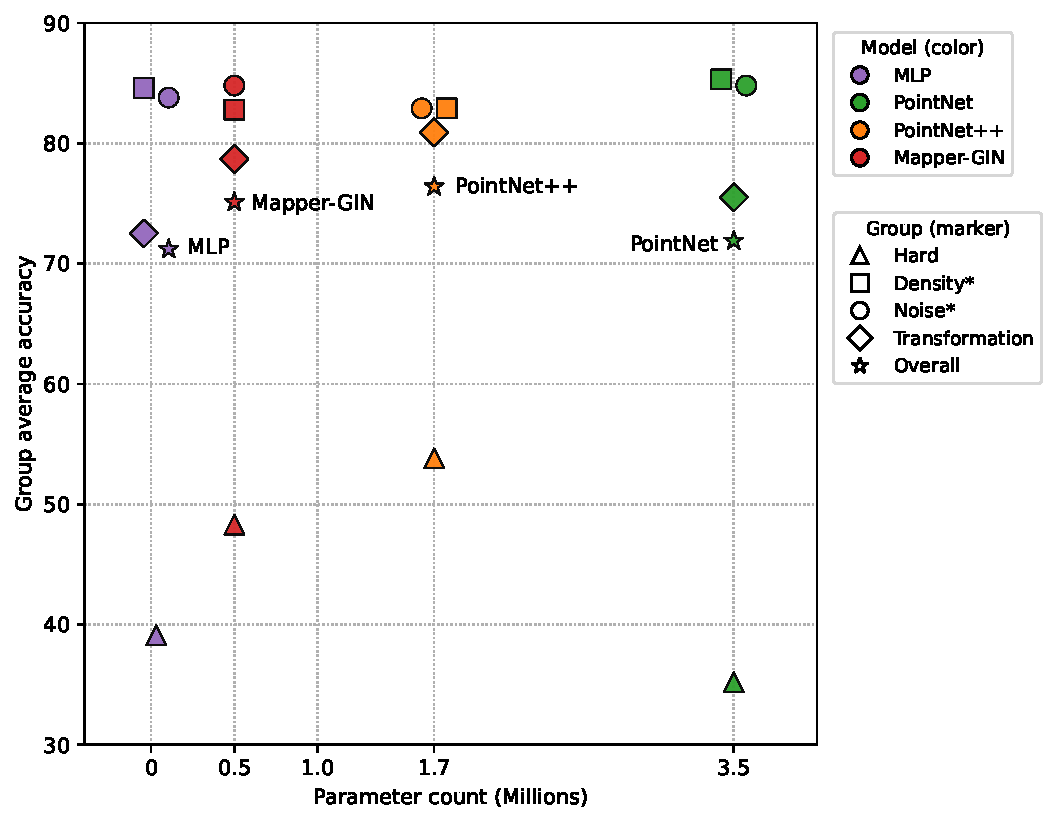
\includegraphics[width=0.5\linewidth]{fig4.pdf}
    \caption{\small Robustness--efficiency tradeoff on ModelNet40-C.}
    \label{fig4}
\end{figure}

\section{Discussion}
Our experiments indicate that region-level structural abstraction can improve corruption robustness in 3D point cloud classification with strong parameter efficiency. Mapper-GIN builds a Mapper-induced region graph and applies GIN message passing on top of a lightweight local encoder to perform structure-aware aggregation. This design achieves robustness close to substantially larger models while avoiding robustness-specific training strategies.

The effect of Mapper-based abstraction is corruption dependent. The largest benefits appear when the induced region graph remains relatively stable. This happens when corruptions do not strongly disrupt the cover assignment and clustering, or when the perturbation is approximately topology-preserving. This helps mitigate local outliers in Noise settings and geometric distortions under Transformations, consistent with Mapper-GIN’s competitive robustness across both regimes.

At the same time, Mapper-GIN shows clear limitations under point-removal regimes. Performance drops more on Density decrease and Cutout than for purely pointwise baselines such as PointNet and MLP. A plausible explanation is that point removal changes cover intersections and local connectivity, modifying the induced region graph topology. When the graph structure shifts, node embeddings become less consistent across severity levels.

From a practical perspective, Mapper introduces additional design choices. The region graph depends on the lens selection, cover resolution, overlap ratio, and clustering. We used fixed graphs computed offline to isolate the effect of structural abstraction. This improves experimental control, but it also means Mapper is not fully end-to-end. Performance can vary with these hyperparameters, so some tuning may be required for new datasets.

Future work could reduce reliance on manual decomposition by making key components of the Mapper pipeline learnable.
In particular, the lens (filter) function could be parameterized as a neural ``learnable lens'' and optimized jointly with the downstream classifier, and the cover/decomposition could be made adaptive within differentiable or optimization-based Mapper formulations \cite{pmlr-v235-oulhaj24a,alvarado2023gmapper}.
Moreover, region assignments could be produced via differentiable or softly-parameterized clustering to replace hard partitions and improve stability under sparsification \cite{genevay2019differentiable}.
Such a partially adaptive construction may allow the induced region structure to adjust to dataset characteristics, potentially retaining the robustness gains observed here while improving usability and flexibility.

\section{Conclusion}

We examined whether topology-inspired region-level structural abstraction can improve robustness in 3D point cloud classification. We proposed Mapper-GIN, which converts a point cloud into a Mapper-induced region graph and applies GIN-based message passing on top of a lightweight point encoder. The model uses a simple Mapper construction (PCA lens, cubical cover, and density-based clustering) and aggregates information over region adjacencies. This design separates point-level encoding from structural aggregation and enables controlled evaluation against a pointwise MLP baseline.

Experiments on ModelNet40-C show that Mapper-GIN achieves competitive robustness with a compact model size. It matches or approaches the robustness of larger architectures while using far fewer parameters and without robustness-specific training. It is particularly effective under noise and transformation corruptions, where regionization and graph aggregation reduce sensitivity to local outliers and geometric distortions. Overall, our results indicate that coarse region graphs provide a practical and interpretable structural prior for robustness, offering a favorable robustness–efficiency tradeoff. These results also reveal limitations when point removal alters the induced region graph, motivating future work on learnable or adaptive Mapper components such as parameterized learnable lenses and differentiable or softly-parameterized clustering.

\bibliographystyle{unsrt}  
\bibliography{references}  

\newpage
\appendix
\section{Visualization of ModelNet40-C Corruptions}
\label{app:fig_corruptions}
\begin{figure}[H]
    \centering
    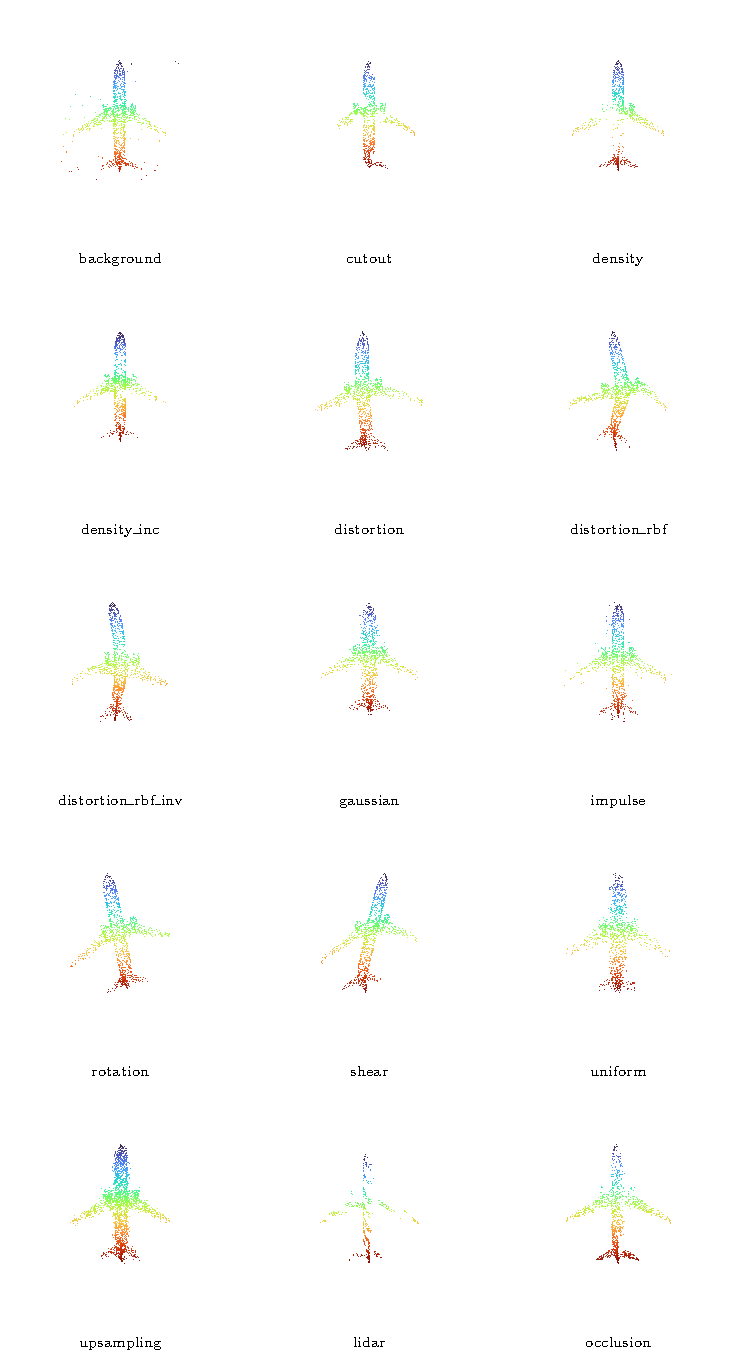
\includegraphics[width=0.65\linewidth]{Appendix/corruption_grid.pdf}
    \caption{\small ModelNet40-C corruptions for an airplane point cloud.}
    \label{fig:Corruptions}
\end{figure}
\end{document}
